\documentclass{article}
\usepackage{graphicx}
\usepackage[margin=1.5cm]{geometry}
\usepackage{amsmath}

\begin{document}

\title{Wednesday Reading Assessment: Unit 5, Field Induction and Inductance}
\author{Prof. Jordan C. Hanson}

\maketitle

\section{Memory Bank}

\begin{itemize}
\item $\epsilon = -L \frac{dI}{dt}$ ... Faraday's law with induction, $L$.  Think of this as the change in voltage across an inductor.
\item Kirchoff's loop rule: the sum of all changes in voltage around a loop in a circuit must be zero.
\end{itemize}

\section{RL Circuits}

\begin{figure}
\centering
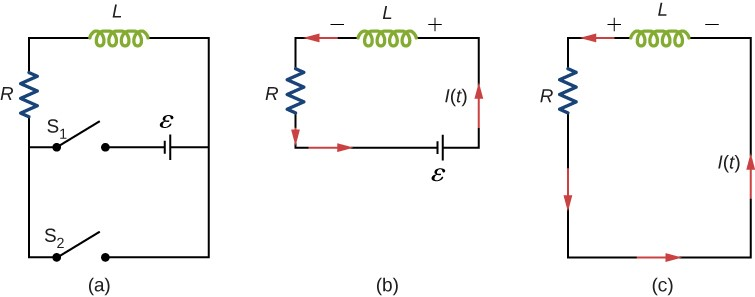
\includegraphics[width=0.5\textwidth]{rl.jpeg}
\caption{\label{fig:rl} A circuit diagram of a DC emf with a resistor, inductor, and two switches.}
\end{figure}

\begin{enumerate}
\item Consider the DC circuit in Fig. \ref{fig:rl}.  There is a battery emf $\epsilon$ connected to a resistor $R$ and and inductor $L$ via switch 1.  Switch 2 simply connects $L$ and $R$.  Suppose we observe the current through the circuit when switch 1 is closed to be
\begin{equation}
i(t) = \frac{\epsilon}{R}\left(1 - \exp(-t/\tau) \right) \label{eq:current}
\end{equation}
(a) Based on Kirchhoff's loop rule, write down the differential equation describes the loop when switch 1 is closed.  Note that $\tau = L/R$.  (b) Plug in Eq. \ref{eq:current} into your differential equation to see if it works. \\ \vspace{3cm}
\item Now we repeat this exercise, but with switch 2 closed and switch 1 opened, after the circuit reaches equilibrium ($t \gg \tau$, when switch 1 was closed).  The equation is observed to be
\begin{equation}
i(t) = \frac{\epsilon}{R}\exp(-t/\tau)
\end{equation}
What formula do we obtain when we apply Kirchhoff's loop rule?  (This is now the situation in part (c) of Fig. \ref{fig:rl}).
\end{enumerate}
\end{document}
